\chapter{Background and Related Work}
\label{cha:background}

This chapter will introduce a concept of containerization, orchestration along with exploring fundamental concepts of the Kubernetes tool, addressing the management of incoming (ingress) and outgoing (egress) traffic within a Kubernetes cluster. Finally, a comparison of selected Container Network Interface plugins will be presented, pointing out their key features. The end will conclude with the literature overview.


%---------------------------------------------------------------------------
\section{Basics}
\label{sec:basics}

In this section, two key Kubernetes concepts will be outlined: containerization and orchestration, showing their roles and benefits in application deployments. These concepts are fundamental for managing modern large-scale environments containing distributed systems.

\subsection{Containerization}
\label{sec:containerization}

Containerization is packaging an application along with all the necessary runtime stuff, like libraries, executables or assets into an object called a "container". The main benefits of containers are \cite{RedhatContainerization}: 

\begin{itemize} 
    \item Portable and Flexible -- a container can be run on bare metal or a virtual machine in the cloud, regardless of the operating system. Only container runtime software, like Docker Engine or \textit{containerd} is required, which allows interacting with the host system. 

    \item Lightweight -- a container shares the operating system kernel with the host machine, so there is no need to install a separate operating system inside. 

    \item Isolated -- it does not depend on the host's environment or infrastructure. 

    \item Standardized -- the Open Container Initiative standardizes runtime, image, and distribution specifications. 
\end{itemize}


A container image is a set of files and configuration needed to run a container. It is immutable, only new images can be created with the latest changes. The layer contains one modification made to an image. All layers are cacheable and can be reused when building an image. The mechanism is useful when compiling large application components inside one container \cite{DockerDocs}. 

%---------------------------------------------------------------------------

\subsection{Container orchestration}
\label{sec:ContainerOrchestration}

Container orchestration is coordinated deploying, managing, networking, scaling, and monitoring containers processes. It automates and manages the whole container's lifecycle, there is no need to worry about the deployed application. Orchestration software like Kubernetes will take care of the availability \cite{RedhatContainerization}.

K8s (Kubernetes) is an open-source orchestration platform capable of managing containers. Key functionalities are \cite{KubernetesDocs}:

\begin{itemize}
    \item Automated rollouts and rollbacks -- updates or downgrades the version of deployed containers at a controlled rate, replacing containers incrementally.
    \item Automatic bin packing -- allows specifying the exact resources needed by a container (CPU, memory) to fit on the appropriate node.
    \item Batch execution -- makes it possible to create sets of tasks that can be run without manual intervention.
    \item Designed for extensibility -- permits adding features using custom resource definitions without changing the source code.
    \item Horizontal scaling -- scales (replicates) the application based on its need for resources.
    \item IPv4/IPv6 dual-stack -- allocates either IPv4 or IPv6 to pods and services.
    \item Secret and configuration management -- allows storing, managing, and updating secrets. Containers do not have to be rebuilt to access updated credentials.
    \item Self-healing -- restarts crashed containers or those that fail as specified by the user.
    \item Service discovery and load balancing -- advertises a container using its DNS name or IP and load balances traffic across all pods in the deployment.
    \item Storage orchestration -- mounts the desired storage, like local or cloud-provided storage, and makes it available for containers.
\end{itemize}
Understanding Kubernetes workflow becomes significantly easier by familiarizing yourself with its architecture, which will be discussed in the following section.


%---------------------------------------------------------------------------

\section{Kubernetes architecture}
\label{sec:k8s_arch}
A Kubernetes cluster is a group of machines that run containers and provide all the necessary services to enable communication between containers within the cluster, as well as access to the cluster from the outside. There are two types of components, the control plane and worker nodes. A minimum of one of each is needed to run a container, but to provide a more robust and reliable production cluster, it is better to use two to three control plane nodes  \cite{KubernetesDocs}. 

\begin{figure}[tbh]
    \centering
    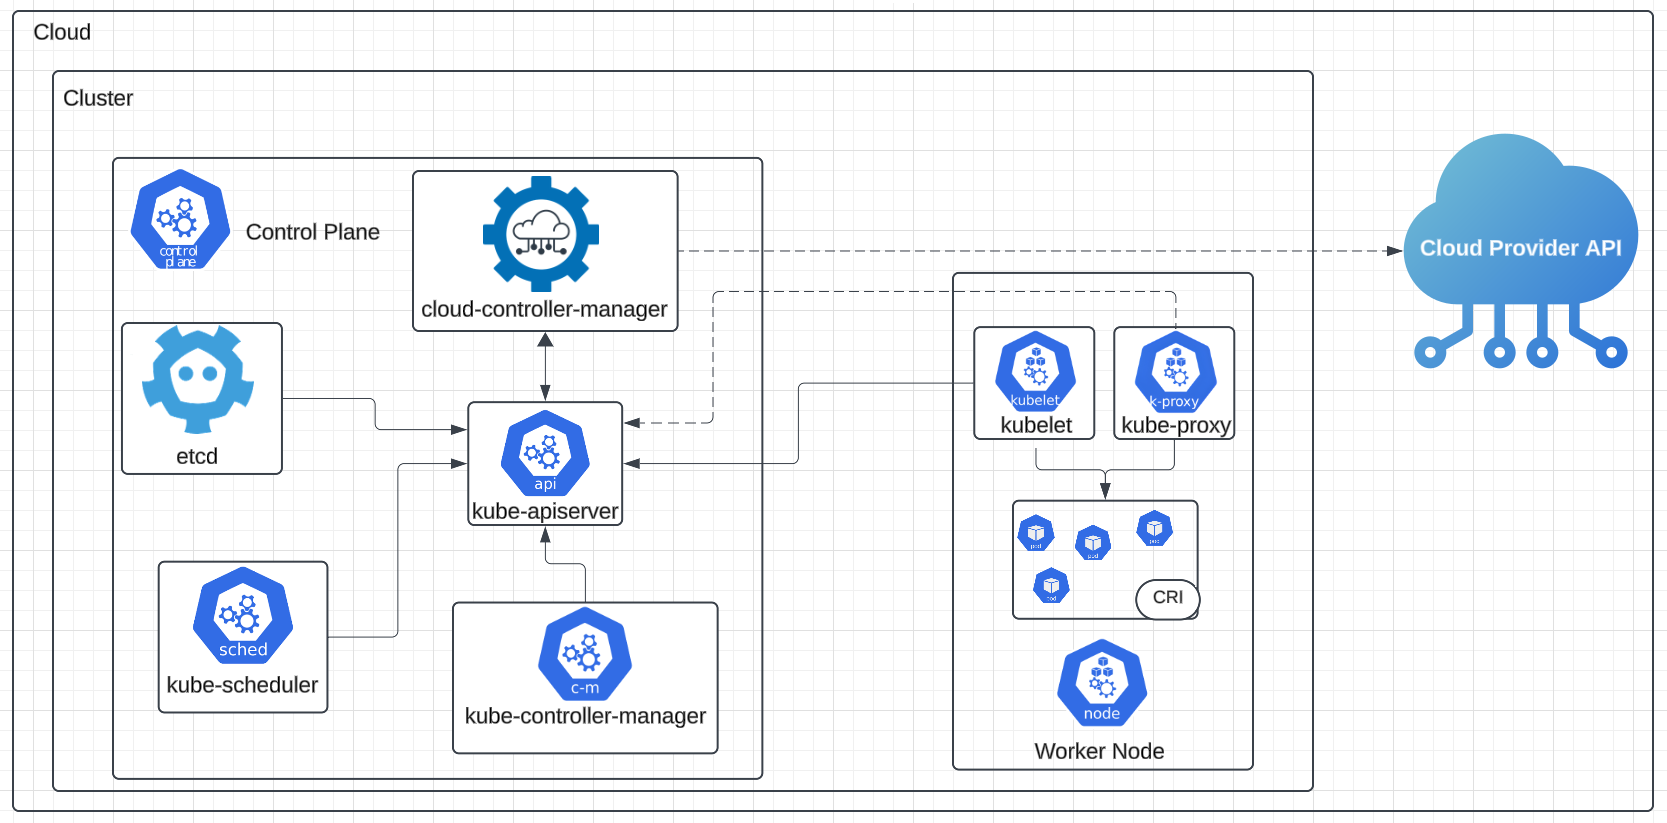
\includegraphics[width=1\columnwidth]{images/kubernetes-cluster-architecture.png}
    \caption{Kubernetes Cluster Architecture \cite{KubernetesDocs}.}
    \label{fig:k8s_arch}
\end{figure}

In Figure~\ref{fig:k8s_arch} there is graphical representation of a Kubernetes cluster. Not all components shown in the figure are mandatory for Kubernetes to work correctly. In the control plane part, \textit{\nameref{sec:cloudControllerManager}} might not be mandatory, in on-premises configurations where interacting with a cloud provider is not needed. On the right side of the figure, in node representation, is the \textit{\nameref{sec:kubeProxy}} component, which is not mandatory, as some networking plugins can provide own implementation of a proxy. This is an example of "Designed for extensibility", where Kubernetes can acquire 3rd-party features without changing its source code \cite{KubernetesDocs}.


%---------------------------------------------------------------------------



\subsection{Control plane}
\label{sec:k8s_cplane}

Control plane is like the brain in the Kubernetes cluster. Interaction with cluster using the \textit{kubectl} tool to perform requests is handled by the \textit{\nameref{sec:kubeApiServer}}. It is responsible for communication with the worker nodes running pods, the smallest unit managed by K8s, which contains containers inside \cite{KubernetesDocs}.

%---------------------------------------------------------------------------

\subsubsection{cloud-controller-manager}
\label{sec:cloudControllerManager}

This component allows Kubernetes clusters to interact with the cloud provider's API. It is combined with the \textit{kube-controller-manager} as single binary and can be replicated. This is the only component that talks to the cloud provider, separating other components from direct communication with the cloud. When running without a cloud environment, this component is absent \cite{KubernetesDocs}.

%---------------------------------------------------------------------------

\subsubsection{etcd}
\label{sec:etcd}

\textit{Etcd} is an open-source distributed key-value store service often used in distributed systems. It is responsible for maintaining both the current state and its previous version in its persistent memory \cite{KubernetesDocs}\cite{Etcd}.

%---------------------------------------------------------------------------

\subsubsection{kube-apiserver}
\label{sec:kubeApiServer}

Exposes Kubernetes API to interact with the cluster. Takes responsibility for handling all requests from components and users. This is the component which answers cluster administrator's requests sent by \textit{kubectl} \cite{KubernetesDocs}.

%---------------------------------------------------------------------------

\subsubsection{kube-controller-manager}
\label{sec:kubeControllerManager}

Component which runs controller processes. Its compiled binary consists of multiple controllers. Example controllers are \cite{KubernetesDocs}:

\begin{itemize}
    \item Node controller -- observes worker nodes if are up and running,
    \item Job controller -- responsible for batch execution jobs,
    \item EndpointSlice controller -- connects services with pods.
\end{itemize}

%---------------------------------------------------------------------------

\subsubsection{kube-scheduler}
\label{sec:kubeScheduler}

Takes care of pods which are not assigned to a worker node yet. \textit{kube-scheduler} is looking for a node that meets the pod's scheduling requirements and fits the pod on that node. Such a node is called feasible node \cite{KubernetesDocs}.

%---------------------------------------------------------------------------

\subsection{Nodes}
\label{sec:k8sNodes}
All the below-mentioned components run on every node in a cluster.
%---------------------------------------------------------------------------

\subsubsection{Container runtime}
\label{sec:containerRuntime}

Node's key component, has ability to run, execute commands, manage, and delete containers in efficient way \cite{KubernetesDocs}. 

%---------------------------------------------------------------------------


\subsubsection{kube-proxy}
\label{sec:kubeProxy}

Create networking rules, which allow communicating with pods from outside the cluster. If available, \textit{kube-proxy} uses the operating system's packet filtering to create a set of rules. It is also able to forward traffic by itself. This component is optional, can be replaced with a different one, if the desired one implements key features \cite{KubernetesDocs}.

%---------------------------------------------------------------------------

\subsubsection{kubelet}
\label{sec:kubelet}

It is responsible for managing containers inside pod on its node. Uses Container Runtime Interface to communicate with containers \cite{KubernetesDocs}.

%---------------------------------------------------------------------------

\subsection{Objects}    
\label{sec:k8s_objects}

\subsubsection{Namespace}
\label{sec:namespace}

The purpose of the namespace object is to isolate groups of resources like pods, deployments, services etc. in a cluster. It helps organize clusters into virtual sub-areas of working space. If a \textit{\nameref{svc}} is created in some custom namespace <service-name>.<namespace-name>.svc.cluster.local DNS entry within cluster is created \cite{KubernetesDocs}.

\subsubsection{Pods}
\label{sec:pods}

Pods are the smallest deployable objects in Kubernetes. They contain one or more containers, which can communicate with each other using the localhost interface. Because they share IP addresses, they cannot use the same ports. It is useful when our service consists of two applications coupled together. For example, there is a pod which has two containers, one responsible for compiling code, the second one is creating a cache entry from compiled object and uploading it to some data storage. It is more logical to share data among containers in a pod than on the node between pods, as it is easier. Scaling is simpler, as it involves replicating a single pod instead of managing two separate pods. Moreover, communication between applications happens using the localhost interface. In scenario where there are two pods, each with one container, ClusterIP \textit{\nameref{svc}} is usually implemented. However, the most common approach is to run one container per pod, where the pod is just managing wrapper for the containerized application. Also, rather than creating pod directly it is more common to use workload resource like \textit{\nameref{deployment}} \cite{KubernetesDocs}. 


\subsubsection{ReplicaSet}
\label{replicaset}

Basically \textit{\nameref{replicaset}} consists of pod template and runs desired number of pods \cite{KubernetesDocs}. 


\subsubsection{Deployment}
\label{deployment}

Deployment is a higher-level abstraction over the \textit{\nameref{replicaset}}, that manages its lifecycle. It provides more features like rolling back an application, as it keeps history of configurations \cite{KubernetesDocs}.

\subsubsection{DaemonSet}
\label{daemonset}

Running pods using a DaemonSet guarantees that every node will have a copy of the desired pod (if resource requirements are met etc.). It can automatically add or remove pods if the number of nodes changes. A typical usage is creating monitoring pods on every node \cite{KubernetesDocs}. 


\subsubsection{StatefulSet}
\label{statefulset}

StatefulSet, unlike a \textit{\nameref{deployment}}, is stateful. It saves an identity of each pod, and if, for example, some persistent storage is assigned to specific database pod. When it dies, Kubernetes will recreate the pod on the same node as before \cite{KubernetesDocs}.

\subsubsection{Job}
\label{job}

Runs a pod that does one task and exists. Kubernetes will retry execution if the pod fails specific number of tries set in its configuration \cite{KubernetesDocs}.

\subsubsection{CronJob}
\label{cronjob}
Behaves like a \textit{\nameref{job}} but can regularly run at specified intervals for tasks like database backups or log rotation \cite{KubernetesDocs}. 

\subsubsection{Service}
\label{svc}

Service exposes an application running inside a cluster by using an endpoint. As a pod is ephemeral resource and its address changes sometimes (e.g., when pod is recreated), it is better to create a DNS name that resolves IP address. Moreover, the service will not advertise unhealthy pods. Usually, a service exposes one port per service, but for example web app might expose HTTP and HTTPS ports. There are four types of services \cite{KubernetesDocs}. 


\begin{enumerate}
    \item ClusterIP -- makes one pod available to other inside cluster by exposing an application using inter-cluster IP address. Although it is oriented to be accessible within the cluster, objects like \textit{\nameref{ingress}} or \textit{\nameref{gatewayapi}} can expose the service to the outside.
    \item NodePort -- by default allocates a port (from range 30000-32767) to publish the service on every node's IP address. In this scenario, every node on the specified port acts like a proxy to the deployed application.
    \item LoadBalancer -- Kubernetes does not provide a load balancer by default. When creating such a service, it interacts with the cloud provider to create an external service for traffic balancing. A load balancer can be installed inside the cluster.
    \item ExternalName -- allows pods inside Kubernetes to access an external service using a defined name, rather than using an IP address 
\end{enumerate}

%---------------------------------------------------------------------------



\subsection{Cluster networking}
\label{sec:k8s_networking}

Networking is the most important thing in Kubernetes, the whole point is to obtain reliable and robust communication among containers, pods, services, nodes, and external systems in a cluster \cite{KubernetesDocs}. There are four types of network communication \cite{KubernetesDocs}:

\begin{enumerate}
    \item container-to-container -- communicates by sharing network resources inside a pod;
    \item pod-to-pod -- every pod can communicate with any other pod without the need to use NAT, as every of them has its own IP address \cite{IBMKubernetesNetworking};
    \item pod-to-service -- covered by service type ClusterIP, which provides an inter-cluster IP address;
    \item external-to-service -- held by services type NodePort and Loadbalancer, which expose pods to the outside.
\end{enumerate}
Kubernetes allocates IP addresses to nodes, services, and pods \cite{KubernetesDocs}:
\begin{itemize}
    \item \textit{\nameref{sec:kubelet}} or \textit{\nameref{sec:cloudControllerManager}}, depending on local or cloud infrastructure allocates IP address for nodes
    \item \textit{\nameref{sec:kubeApiServer}} allocates the IP address for services
    \item the allocation of an IP address to a pod is the managed by the networking plugin, which is an implementation of \textit{\nameref{sec:cni}}.
\end{itemize}


%---------------------------------------------------------------------------

\section{The concept of traffic engineering in Kubernetes}
\label{sec:trafficConcept}

Traffic Engineering is a key concept in Kubernetes to provide production-ready, reliable, and efficient network. In this section ingress and egress traffic will be explained.

%---------------------------------------------------------------------------

\subsection{Ingress traffic management}
\label{sec:ingressTrafficMngmnt}

\subsubsection{Ingress}
\label{ingress}

Ingress is an object that manages outside the cluster access to services inside the cluster. It is a single point of entry to route traffic to specified pod based on configuration. This is only a higher abstract object that specifies routing rules in the cluster. Real functionalities are provided by an \textit{\nameref{ingresscontroller}}. Nowadays the development on Ingress is frozen, Kubernetes authors pay attention to its successor, the \textit{\nameref{gatewayapi}} \cite{KubernetesDocs}.

\subsubsection{Ingress Controller}
\label{ingresscontroller}

An Ingress Controller fulfills an \textit{\nameref{ingress}} and starts serving an application which performs configured rules. Any implementation has its own features, but common functionalities are L4/L7 load balancing, host and path-based routing, SSL termination. This is the real application that runs in a pod. Ingress Controller must be installed manually and is not part of Kubernetes, however the container orchestration tool developers maintain AWS, GCE, and nginx ingress controllers \cite{KubernetesDocs}. 


\subsubsection{Gateway API}
\label{gatewayapi}

The functionalities of the Gateway API are so wide, that the Kubernetes authors use term "project". The project focuses on L4 and L7 routing in a cluster. It succeeds \textit{\nameref{ingress}}, Load Balancing and service mesh APIs. The Gateway API resource model is role-oriented \cite{KubernetesGatewayAPI}.

\begin{figure}[tbh]
    \centering
    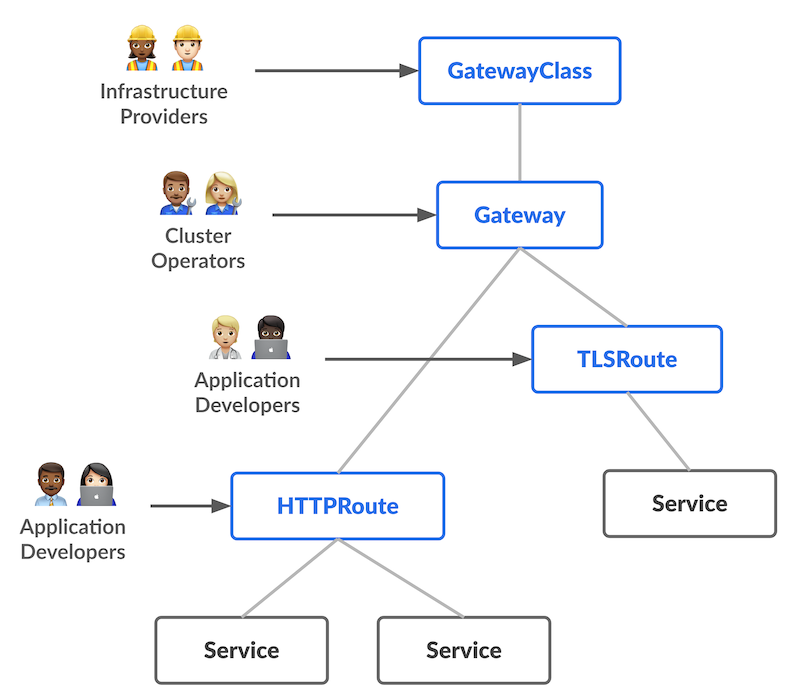
\includegraphics[width=0.7\columnwidth]{images/gateway-api-resource-model.png}
    \caption{Gateway API roles-oriented resource model \cite{KubernetesGatewayAPI}.}
    \label{fig:gatewayApiResourceModel}
\end{figure}

The model focuses on three separate groups of people who interact with a cluster on various levels. 

On a top of Figure~\ref{fig:gatewayApiResourceModel} there are infrastructure providers, who provide the GatewayClass resource. They are responsible for the overall multiple clusters, rather than ensuring developers can access pods correctly \cite{KubernetesGatewayAPI}. The GatewayClass resource is a class of Gateway which can be created. It defines specific types of load balancing implementations and provides clear explanation of capabilities available in the Kubernetes resource model. The functionality is like \textit{\nameref{ingress}}. There can be more than one GatewayClasss created \cite{KubernetesGatewayAPI}. 


Cluster operators are in the middle of Figure~\ref{fig:gatewayApiResourceModel}, they make sure that cluster meets requirements for several users. As maintainers define the Gateway resource, some load balancing system is provisioned by the GatewayClasss. The Gateway resource defines a specific instance which will handle incoming traffic. Allows defining the specific protocol, port or allowed resources to route inbound traffic \cite{KubernetesGatewayAPI}.

End users specified in the Gateway API resource model in Figure~\ref{fig:gatewayApiResourceModel} are the application developers. They focus on serving applications to the clients by creating a resource named HTTPRoute. The resource defines HTTP routing from defined gateway to end API objects like service. It can to split traffic using "weight" as a key, which represents the percentage of the total traffic to be routed. The GRPCRoute is similar, but operates on different protocol \cite{KubernetesDocs}\cite{KubernetesGatewayAPI}. 



The Gateway API is not an API Gateway. An API Gateway in general is responsible for routing, load balancing, information exchange manipulation and much more depending on specific implementation. The Gateway API is set of three resources mentioned earlier, which creates a role-oriented Kubernetes service networking model. Creators of the Gateway API provide a clear explanation: "Most Gateway API implementations are API Gateways to some extent, but not all API Gateways are Gateway API implementations" \cite{KubernetesGatewayAPI}. 

%---------------------------------------------------------------------------

\subsection{Egress traffic management}
\label{sec:egressTrafficMngmnt}

Egress traffic refers to connections which leave cluster and are initiated inside by pods. In contrast to the Ingres object, in Kubernetes there is no Egress resource, outgoing traffic route logic is implemented by Container Network Interface plugin. The most common approach in managing egress traffic is to use Kubernetes Network Policies to deny all outgoing traffic and then allow only key connections. The limitation is that all external services need to be specified with IP address in policies. Any change in external resource's IP requires a change in policy configuration. If any pod is trying to access external service, source network access translation (SNAT) needs to be performed to map inter-cluster pod IP to externally routed nodes IP. When the response is accessing cluster, SNAT is performing translation in opposite way. Another key egress concept in Kubernetes is an egress gateway. This is a node which proxies outgoing traffic from a cluster, specified by provided configuration (e.g., by labeling pods, depends on CNI implementation). The important thing is that the internal pod's IP address is masqueraded into IP address of an egress gateway, outside peer does not see ephemeral IP of a pod. Egress gateway is also a CNI specific implemented resource \cite{CalicoDocs}\cite{CiliumDocs}. 


%---------------------------------------------------------------------------

\section{Container network interface (CNI)}
\label{sec:cni}
CNI is standardized by Cloud Native Computing Foundation set of API rules which defines container networking. CNI is responsible for pod-to-pod communication, which includes assigning IP addresses, configuring network interface inside container and routing \cite{IBMKubernetesNetworking}. 



%---------------------------------------------------------------------------

\subsection{Overview of selected CNI plugins}
\label{sec:cni_overview}


\begin{table}[h!]
    \centering
    \caption{Comparison of Antrea and Cilium \cite{CiliumDocs}\cite{AntreaDocs}.}
    \resizebox{\textwidth}{!}{%
    \begin{tabular}{|l|l|l|}
    \hline
    \textbf{Feature/Plugin}              & \textbf{Antrea}                                         & \textbf{Cilium}                                \\ \hline
    \textbf{Dataplane}            & Open vSwitch                                            & eBPF                                           \\ \hline
    \textbf{Encapsulation}        & VXLAN or Geneve                                         & VXLAN or Geneve                                \\ \hline
    \textbf{Encryption}           & IPsec or WireGuard tunnels                              & IPsec or WireGuard tunnels                     \\ \hline
    \textbf{Security}             & Extends Kubernetes Network Policies                     & Advanced security policies                     \\ \hline
    \textbf{Observability}        & Theia and Grafana for visualization                     & Hubble                                         \\ \hline
    \textbf{Purpose}              & Simplified Kubernetes networking management             & For large-scale cluters                        \\ \hline
    \textbf{Additional features}  & Network policies for non-Kubernetes nodes               & BGP to advertise network outside cluster       \\ \hline
    \textbf{Gateway API}          & No support                                              & Fully supports Gateway API                     \\ \hline
    \textbf{Egress Gateway}       & Basic egress gateway capabilities                       & Advanced egress gateway support                \\ \hline
    \end{tabular}}
    \label{tab:antrea_cilium}
\end{table}


Antrea is an open-source CNI plugin which is built on Open vSwitch which requires a kernel version greater than 4.6 \cite{AntreaDocs}. OvS is a virtual switch with capability of handling traffic flow between virtual machines and containers \cite{OvS}. Antrea's focus is L3/L4 networking and security services, such as network policies. The resource is responsible for managing traffic flow between pods. By default, every pod can communicate with any other pod, but network policies can specify if pod A is able to talk to pod B \cite{KubernetesDocs}. Consider scenario with three pods, client, frontend, and backend. There is no need to allow a client communication directly with the backend, so network policies allow traffic flow from the client to the frontend and direct communication with the backend is not allowed \cite{CalicoDocs}. 


Cilium, open-source CNI which uses eBPF (extended Barkeley Packer Filter) for packet processing, security and deep observability using Hubble \cite{CiliumDocs}. Some environments may not be suitable because Cilium requires a kernel version of 5.4 or higher \cite{CiliumDocs}. eBPF is a technology that allows running defined programs, with custom logic inside the operating system kernel in a privileged context without requiring of any kernel source code changes or loading modules. The lack of switching between kernel space and user space reduces latency \cite{eBPF}. 

Figure~\ref{fig:ebpf_routing}, shows standard container networking on the left side and Cilium eBPF container networking on the right. The whole point of eBPF networking is skipping overhead that comes from \textit{iptables}. Moreover, eBPF implements hash tables for storing routing policies, which time complexity is O(log n), compared to \textit{iptables} array O(n). It makes clear that large-scale clusters will benefit from using eBPF \cite{IsovalentHash}. 

\begin{figure}[H]
    \centering
    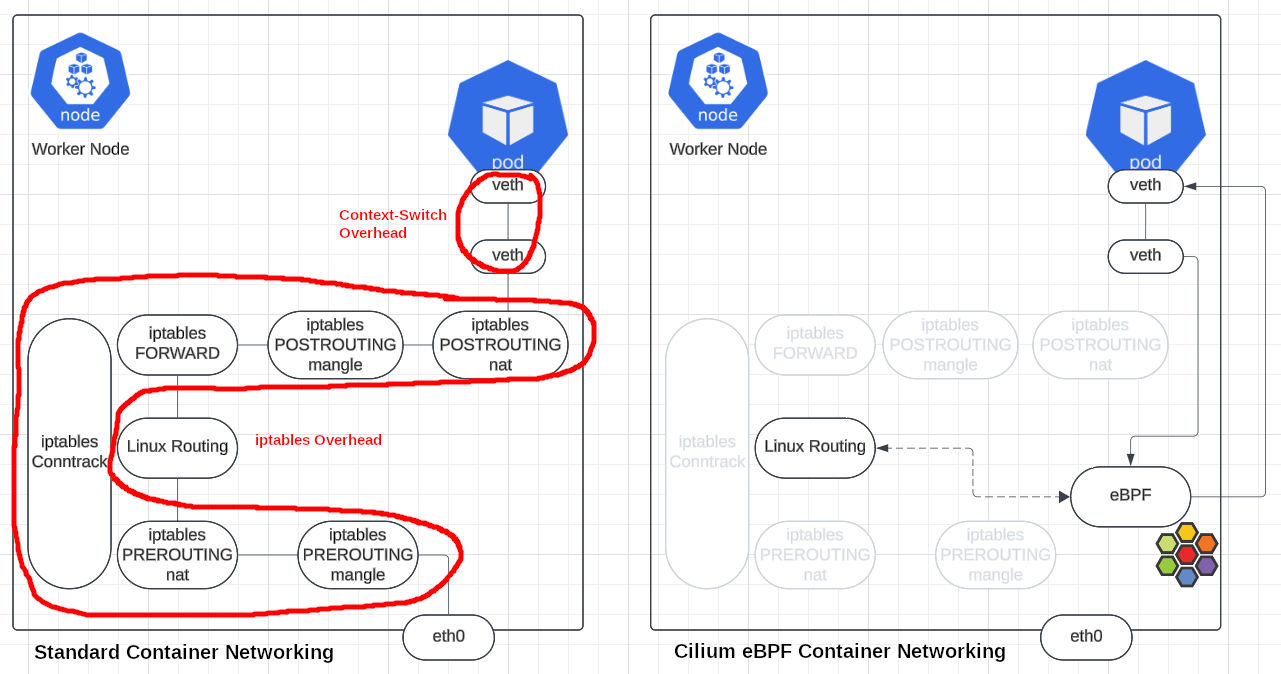
\includegraphics[width=0.9\columnwidth]{images/ebpf_hostrouting.png}
    \caption{Cilium eBPF host-routing \cite{CiliumCNIBenchmark}.}
    \label{fig:ebpf_routing}
\end{figure}



%---------------------------------------------------------------------------

\section{Related work}
\label{sec:realted_work}

As discussed in \cite{dakic2024performance} the performance of different CNIs can vary widely, some CNIs performing two to three times better than others, making it essential to choose the right plugin for a particular workload. Authors say that developing automated methodology of CNI plugin evaluation is a key aspect, specifically in large High-Performance Computing (HPC) environments. This allows for reproducible and consistent tests across different configurations, reducing the overhead of manual testing. To achieve that, tools like Ansible can be helpful. They state that Linux Kernel or NIC can be a bottleneck in networking performance, so they extend maximum buffer size, scale TCP window, disable TCP Selective Acknowledgement, increase SYN Queue Size, or enable Generic Receive offload. The paper shows results of comparison four CNI plugins, such as Antrea, Cilium, Calico, Flannel using TCP/UDP in base and with optimized system settings \cite{dakic2024performance}. 

In \cite{9153266} the authors measure CNI plugins for inter-host and intra-host communication using UDP and TCP protocols. They introduce the concept of CPU cycles per packet (CPP) to evaluate CNI efficiency. They measure CPP spent in each network component using the Linux \textit{perf} tool. By measuring throughput, RTT, and latency, they compare how different CNI plugins (Flannel, Weave, Cilium, kube-router, Calico) compared to its network models \cite{9153266}. 

In a paper, the same authors as before focus on functionality, performance, and scalability. They scale testbed up to 99 \textit{Iperf} client and 99 \textit{Iperf} server pod, mentioning that 100 pods is a limit for Kubernetes node \cite{9309003}. 

The authors of \cite{10138542} state that in the coming years, fifth generation mobile networks (5G) will deploy a significant part of their infrastructure in the cloud-native platforms, resulting in the creation of large-scale clusters. Such production environments containing thousands of pods require creating stable, reliable, and efficient networks. They do not focus their attention on which CNI uses in this scenario, rather highlight such concepts as highly performant networking, security, and observability. Authors state that the key to meet this expectation is eBPF (extended Barkeley Packet Filter) \cite{10138542}. 
